\section{Specifications}

\noindent
The syntax of  \SpecLang specifications is given below
 
\begin{definition}  

\noindent
{\emph{{Syntax of \SpecLang Specifications}}}

\label{f:holistic-syntax}
\[
\begin{syntax}
\syntaxElement{S}{}
		  {\syntaxline
                               {\OneStateQ {\overline {x:C}} {A} }	
				{\TwoStatesQ {\overline {x:C}} {A} {A} }	
				{S\, \wedge \, S}
		 \endsyntaxline
		}
\endSyntaxElement\\
\end{syntax}
\]
\end{definition}


\subsubsection{Arising States} % and {Arising} External States}
\footnoteSD{TODO motivate;
Here what we had: As discussed in \S \ref{s:approach}, 
{open world specifications need to be able to provide}
guarantees which hold
during execution of an internal, 
known, trusted module $M$ when linked together with any
unknown, untrusted, module $M_{ext}$. These guarantees need only hold 
when the external module is executing; we are not concerned if they are
temporarily broken by the internal module. Therefore, we are only interested in states where the
executing object (\prg{this}) is an external object. 
To express our focus on external states, we define the  \emph{external states semantics}, of the form 
$\reduction{M_{ext}}{M}{\sigma}{\sigma'}$, where $M_{ext}$ is the external
module, and $M$ is the internal module, and where we
collapse all internal steps into one single step.
}
{A state $\sigma$ is \emph{arising},}  written $\arising{\sigma}{M}$, {if it  may arise}  % by observable states} 
by execution
starting at some initial configuration:


\begin{definition}[Arising  States]
\label{def:arising}
For modules $M$ and $M_{ext}$ we define arising and arising external states as follows:

\begin{itemize}
\item
 a state $\sigma$ is 
{ an \emph{arising} state, formally \ \ \  $\arising{\sigma}{M}$,\ \ \ if  there exists some $\sigma_0$ such that $\initial{\sigma_0}$ and
$M, {\sigma_0} \leadsto^* {\sigma}$.}
%\item
%{A a state $\sigma$ is 
%called an \emph{arising} state, formally\ \ \ \  $\extArising{\sigma}{M_{ext}}{M}$,\ \ \ \
%if and only if $\arising{\sigma}{M_{ext}*M}$ and $M, \sigma \models \external{\prg{this}}$.}
\end{itemize}
\end{definition}


An \emph{Initial} state's heap contains a single object of class \prg{Object}, and
its  stack   consists of a single frame, whose local variable map is a
mapping from \prg{this} to the single object, and whose continuation is  any statement.
(See Definition %s \ref{def:initial} and 
\ref{def:arising} and the 
{appendices %of the full paper 
\cite{necessityFull}).}


 
 \subsubsection{ Semantics of \SpecLang Specifications}
We now  define what it means for  a module  $M$ to satisfy specification  $S$, written as $M \vDash S$. The
 
\begin{definition}% [Semantics of \SpecLang Specifications]

We define $\satisfies{M}{{S}}$ by cases over the three possible syntactic forms.
For any assertions   $A_1$, $A_2$, and $A$: \\

\label{def:necessity-semantics}

\begin{tabular}{l l c l }

$\bullet$ & $\satisfies{M}{\OneStateQ {\overline {x:C}} {A} 	}$& iff & 
for all $M_{ext}$, $\sigma$, $\overline{x}$, such that $\overline{x}$  are free in $\sigma$, \\
  & & & $ \arising{\sigma}{M_{ext}\!\circ \! M}  \ \  \wedge\ \ M, \sigma  \models {\external{\prg{this}}} % \ \wedge 
$\\
& & & $ \ \Longrightarrow \  $ \\ % \\ & & &  $ \satisfiesA{M}{\sigma[\overline{x\mapsto o}]}{A} $
& & &  {$ \satisfiesA{M}{\sigma}{\forall \overline{x:C}.A}$}
\\
\\
$\bullet$ & $\satisfies{M}{\TwoStatesQ {\overline {x:C}} {A}{A'}}$& iff & 
for all $M_{ext}$, $\sigma$, $\overline{x}$, $\overline{o}$ such that $\overline{x}$  are free in $\sigma$  \\
 & & & $ \arising{\sigma}{M_{ext}\!\circ \! M}\   \  \wedge\ \ M, \sigma  \models {\external{\prg{this}}}  
\ \ \wedge $
\\
 & & & $\GRelevant {\overline o}  \sigma \ \ \wedge\ \    \satisfiesA{M}   {\sigma[\overline{x\mapsto o}]}{(\overline {x:C} \wedge A)} \ \ \wedge$ \\ 
 & & & $\red{\leadstoBoundedStar {M_{ext}\!\circ \!M}{\sigma}{\sigma} {\sigma'} } \ \ \wedge\ \  M, \sigma' \models {\external{\prg{this}}}$ \\
& & & $ \Longrightarrow $ \\
& & & $ \satisfiesA{M}{\sigma'[\overline{x\mapsto o}]}{A'} $
\\
\\
$\bullet$ &  $\satisfies{M}{S\, \wedge\, S'}$ &   iff   & $\satisfies{M}{S}\ \wedge \ \satisfies{M}{S'}$
\end{tabular} 

 
\end{definition} 


\footnoteSD{First bullet: This means that we require all objects to satisfy even if not locally relevant. Second Bullet: notice that we are asking for globally relevant objects}  
\footnoteSD{{TODO: Make an example that demonstrates the difference if in the second bullet we had asked for locally relevant objects ${\overline o}$.}}
\footnoteSD{{TODO Notice that we assume that $\overline x$ are not free in $A$ -- cf Barendregt convention.}}
\footnoteSD{TODO: explain why we did not require the stronger $\leadstoFin{M_{ext}\!\circ \!M}{\sigma}{\sigma'}$ rather than $\leadstoBoundedStar {M_{ext}\!\circ \!M}{\sigma}{\sigma} {\sigma'}$.}
% Note that the requirements that $\extArising{\sigma}{M_{ext}}{M}$ and $\leadstoFin{M_{ext}\circ M}{\sigma}{\sigma'} $ imply that
% $M, \sigma' \models {\external{\prg{this}}}$



\sdN{We demonstrate the meaning of ${\TwoStatesQ {\overline {x:C}} {A_0}{A_0}}$ in Fig. \ref{fig:illusrPreserve} where we refine the execution shown in Fig. \ref{fig:UpSemantics}, and take it that the pink states, \ie   ${\sigma_6}$-${\sigma_9}$ and $\sigma_{13}$-$\sigma_{17}$, and  $\sigma_{20}$, $\sigma_{21}$ are external, and the green states, \ie   ${\sigma_{10}}$,  ${\sigma_{11}}$,   ${\sigma_{12}}$,  ${\sigma_{18}}$, and  ${\sigma_{19}}$, are internal.}
 
 \begin{figure}[htb]
\begin{tabular}{|c|}
\hline  % \\
\resizebox{6cm}{!}{
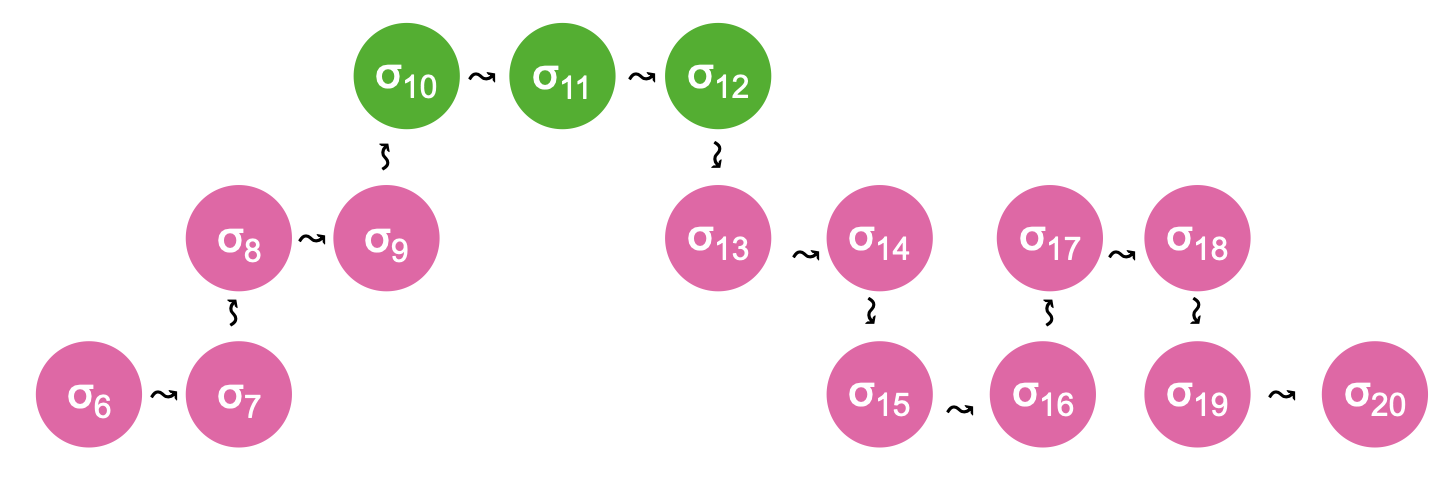
\includegraphics[width=\linewidth]{diagrams/preserves.png}, 
} 
\\
\hline
% \\
\begin{tabular}{lclclcl} 
$ {\sigma_6} \leadsto^*  \sigma_9 $ preserves $A_0$ & &
$ {\sigma_6} \leadsto^*  \sigma_{10} $ does not preserve $A_0$ \\
$ {\sigma_8} \leadsto^*  \sigma_{14} $ preserves $A_0$ & &
$ {\sigma_8} \leadsto^* \sigma_{17} $ does not preserve $A_0$\\
$ {\sigma_7} \leadsto^*  \sigma_{16} $  preserve $A_0$ & &
$ {\sigma_9} \leadsto^*  \sigma_{19} $ does not preserve $A_0$
\\
\hline
\end{tabular}
\end{tabular}
   \caption{Illustrating  the meaning on ${\TwoStatesQ {\overline {x:C}} {A_0}{A_0}}$  -- refining Fig. \ref{fig:UpSemantics}.  }
   \label{fig:illusrPreserve} 
 \end{figure}
 
\subsection{Specification Examples}
\noindent
As an example, consider the following    specifications:

\begin{tabular}{lcll}
$S_1$   &     $\triangleq$   & $\OneStateQ{\prg{a}:\prg{Account} } {\inside{\prg{a}}} $
 \\
 $S_2$   &     $\triangleq$   & $\OneStateQ{\prg{a}:\prg{Account} } {\inside{\prg{a.password}}} $
 \\
 $S_3$   & $\triangleq$   &  $\TwoStatesQ {\prg{a}:\prg{Account}}  {\inside{\prg{a}}} {\inside{\prg{a}}} $
 \\
 $S_4$   & $\triangleq$   &  $\TwoStatesQ {\prg{a}:\prg{Account}}  {\inside{\prg{a.password}}} {\inside{\prg{a.password}}}$
 \\
$S_5$ & $\triangleq$   &
 $\forall \prg{a}:\prg{Account}.\forall \prg{b}:\prg{int}.$\\
  &  &  $\FirstState{\inside{\prg{a}} \wedge \prg{a.balance}=\prg{b}} 
\  \SecondState{ \prg{a.balance}= \prg{b} }$
\\
$S_6$ & $\triangleq$   &
  $\forall \prg{a}:\prg{Account}.\forall \prg{b}:\prg{int}.$\\
  &  &  $\FirstState{\inside{\prg{a.password}} \wedge \prg{a.balance}=\prg{b}} 
\  \SecondState{ \prg{a.balance}\geq \prg{b} }$
 \end{tabular}

\vspace{.2cm}
Now consider our modules from earlier. We have that

\begin{tabular}{lllllll}
$\ModA \not\models S_1$  & & $\ModA \not\models S_2$ &&  $\ModB \not\models S_1$ &  &$\ModB \not\models S_2$ \\
$\ModA \models S_3$ & &   $\ModA \models S_4$ & &  $\ModB  \models S_3$ & &  $\ModB  \not\models S_4$ \\
$\ModA \models S_5$ & &  $\ModA \models S_6$ & & $\ModB  \models S_5$ & & $\ModB   \not\models S_6$ \\
\end{tabular}

\vspace{.6cm}
Consider also  $S_{4a}$ which is a variation of $S_4$, as well as $S_7$, which ...

\begin{tabular}{lcll}
$S_{4a}$   &     $\triangleq$   &   ${\TwoStatesQ {\prg{a}:\prg{Account}.\prg{p}:\prg{Password}}  {\prg{p}=\prg{a.password} \wedge \inside{\prg{p}}}{\inside{\prg{p}}} }$
 \\
$S_7$ & $\triangleq$   & ${\TwoStatesQ {\prg{a}:\prg{Account}.\prg{p}:\prg{Password}}  {\prg{p}=\prg{a.password}} {\prg{p}=\prg{a.password}} }$
 \end{tabular}
 
 \noindent
 Fort these specifications
 
 \begin{tabular}{lllllll}
$\ModA  \models S_7$  & & $\ModB \not\models S_7$ &&  $\ModC \not\models S_7$ \\
\end{tabular}

\subsection{Tautological assertions, and Specification Implication}

\begin{definition}[Satisfaction of Assertions by a module] 
\label{def:assertion-inference-semantics}
We define satisfaction of an assertion $A$ by a  module $M$ as:
\begin{itemize}
\item
$M \vDash A$   \ \ \ iff \ \ \  $\forall M_{ext}. \forall \sigma.[\ \extArising{\sigma}{M_{ext}}{M} \ \Longrightarrow \ \ \satisfiesA{M}{\sigma}{e}\ \ ]$
\end{itemize}
\end{definition}

TODO: Here we will say that assertions are classical, as proven in FASE

\begin{definition}[Stronger Specifications] 
\label{def:specification-implication-semantics}
We define when a specification $S$ is stronger than another specification $S'$  in the context of a  module: 
 \begin{itemize}[itemsep=5pt]
\item 
$\stronger M  S  {S'}$   \ \ \ iff \ \ \  $M\models S$ implies $M \models S'$
\item
$\strongerEq M  S  {S'}$   \ \ \ iff \ \ \ $\stronger M  S  {S'}$  \ and \  $\stronger M   {S'} S$    
\end{itemize}
\end{definition}

We know about stronger specifications:

\begin{lemma}
Consider assertions $A$, $A'$, variable $y$ free in $A$, specifications $S$, $S'$, and module $M$:
\begin{itemize} [topsep=6pt,itemsep=5pt,parsep=0pt,partopsep=0pt]
\item
$\stronger M {\OneStateQ {\overline {x:C}}  {A}}  {\TwoStatesQ {\overline {x:C}} {A}{A}} $ 
    \item
 $\strongerEq  M  {\OneStateQ    {y:\prg{Object}}   {\forall \overline {x:C}[ A ] } } 
    {\OneStateQ {\overline {x:C}}  {A}} $.
\item
$  M  \models (  \overline {x:C} \wedge A) \rightarrow A'$ \ \ \  implies \ \  \ $\stronger M  {\OneStateQ {\overline {x:C}} {A}}    {\OneStateQ {\overline {x:C}} {A'}}$
\item
  \ $\stronger M  { \TwoStatesQ {y:\prg{Object}}  {\forall x:C.[A]} {\forall x:C.[A']} }    {\TwoStatesQ {\overline {x:C}} {A}{A'}} $

\item
$\stronger M  S {S''}$ and $\stronger M {S''} {S'}$\ \  implies \ \ $\stronger M S  {S'}$.
\end{itemize}

\end{lemma}



